\documentclass[11pt, a4paper]{article}
\usepackage{pdfpages}
\usepackage{parallel}
\usepackage[T2A]{fontenc}
\usepackage{ucs}
\usepackage[utf8x]{inputenc}
\usepackage[polish,english,russian]{babel}
\usepackage{hyperref}
\usepackage{rotating}
\usepackage[inner=2cm,top=1.8cm,outer=2cm,bottom=2.3cm,nohead]{geometry}
\usepackage{listings}
\usepackage{graphicx}
\usepackage{wrapfig}
\usepackage{longtable}
\usepackage{indentfirst}
\usepackage{array}
\usepackage{tikzsymbols}
\usepackage{soul}
\usepackage[ruled,vlined]{algorithm2e}
%\counterwithout{figure}{section} 

\usepackage{url}
\makeatletter
\g@addto@macro{\UrlBreaks}{\UrlOrds}
\makeatother

\newcolumntype{P}[1]{>{\raggedright\arraybackslash}p{#1}}
\frenchspacing
\usepackage{fixltx2e} %text sub- and superscripts
\usepackage{icomma} % коскі ў матэматычным рэжыме
\PreloadUnicodePage{4}

\newcommand{\longpage}{\enlargethispage{\baselineskip}}
\newcommand{\shortpage}{\enlargethispage{-\baselineskip}}

\def\switchlang#1{\expandafter\csname switchlang#1\endcsname}
\def\switchlangbe{
\let\saverefname=\refname%
\def\refname{Літаратура}%
\def\figurename{Іл.}%
}
\def\switchlangen{
\let\saverefname=\refname%
\def\refname{References}%
\def\figurename{Fig.}%
}
\def\switchlangru{
\let\saverefname=\refname%
\let\savefigurename=\figurename%
\def\refname{Литература}%
\def\figurename{Рис.}%
}

\hyphenation{admi-ni-stra-tive}
\hyphenation{ex-pe-ri-ence}
\hyphenation{fle-xi-bi-li-ty}
\hyphenation{Py-thon}
\hyphenation{ma-the-ma-ti-cal}
\hyphenation{re-ported}
\hyphenation{imp-le-menta-tions}
\hyphenation{pro-vides}
\hyphenation{en-gi-neering}
\hyphenation{com-pa-ti-bi-li-ty}
\hyphenation{im-pos-sible}
\hyphenation{desk-top}
\hyphenation{elec-tro-nic}
\hyphenation{com-pa-ny}
\hyphenation{de-ve-lop-ment}
\hyphenation{de-ve-loping}
\hyphenation{de-ve-lop}
\hyphenation{da-ta-ba-se}
\hyphenation{plat-forms}
\hyphenation{or-ga-ni-za-tion}
\hyphenation{pro-gramming}
\hyphenation{in-stru-ments}
\hyphenation{Li-nux}
\hyphenation{sour-ce}
\hyphenation{en-vi-ron-ment}
\hyphenation{Te-le-pathy}
\hyphenation{Li-nux-ov-ka}
\hyphenation{Open-BSD}
\hyphenation{Free-BSD}
\hyphenation{men-ti-on-ed}
\hyphenation{app-li-ca-tion}

\def\progref!#1!{\texttt{#1}}
\renewcommand{\arraystretch}{2} %Іначай формулы ў матрыцы зліпаюцца з лініямі
\usepackage{array}

\def\interview #1 (#2), #3, #4, #5\par{

\section[#1, #3, #4]{#1 -- #3, #4}
\def\qname{LVEE}
\def\aname{#1}
\def\q ##1\par{{\noindent \bf \qname: ##1 }\par}
\def\a{{\noindent \bf \aname: } \def\qname{L}\def\aname{#2}}
}

\def\interview* #1 (#2), #3, #4, #5\par{

\section*{#1\\{\small\rm #3, #4. #5}}
\ifx\ParallelWhichBox\undefined%
    \addcontentsline{toc}{section}{#1, #3, #4}%
\else%
\ifnum\ParallelWhichBox=0%
    \addcontentsline{toc}{section}{#1, #3, #4}%
\fi\fi%

\def\qname{LVEE}
\def\aname{#1}
\def\q ##1\par{{\noindent \bf \qname: ##1 }\par}
\def\a{{\noindent \bf \aname: } \def\qname{L}\def\aname{#2}}
}

\newcommand{\interviewfooter}[1]{
\vskip 1em
\noindent \textit{#1}
}

\switchlang{ru}
\begin{document}

\title{2000 "--- мышь SurfMouse}
\date{}
\maketitle
\selectlanguage{russian}
Мышь SurfMouse является характерным примером скевоморфного манипулятора "--- такого, который имитирует внешний вид другого объекта, никак не связанного с его основной функцией. Несложно заметить, что в данном случае копируется внешний вид доски для серфинга (рис. \ref{fig:SurfMousePic}).

\begin{figure}[h]
    \centering
    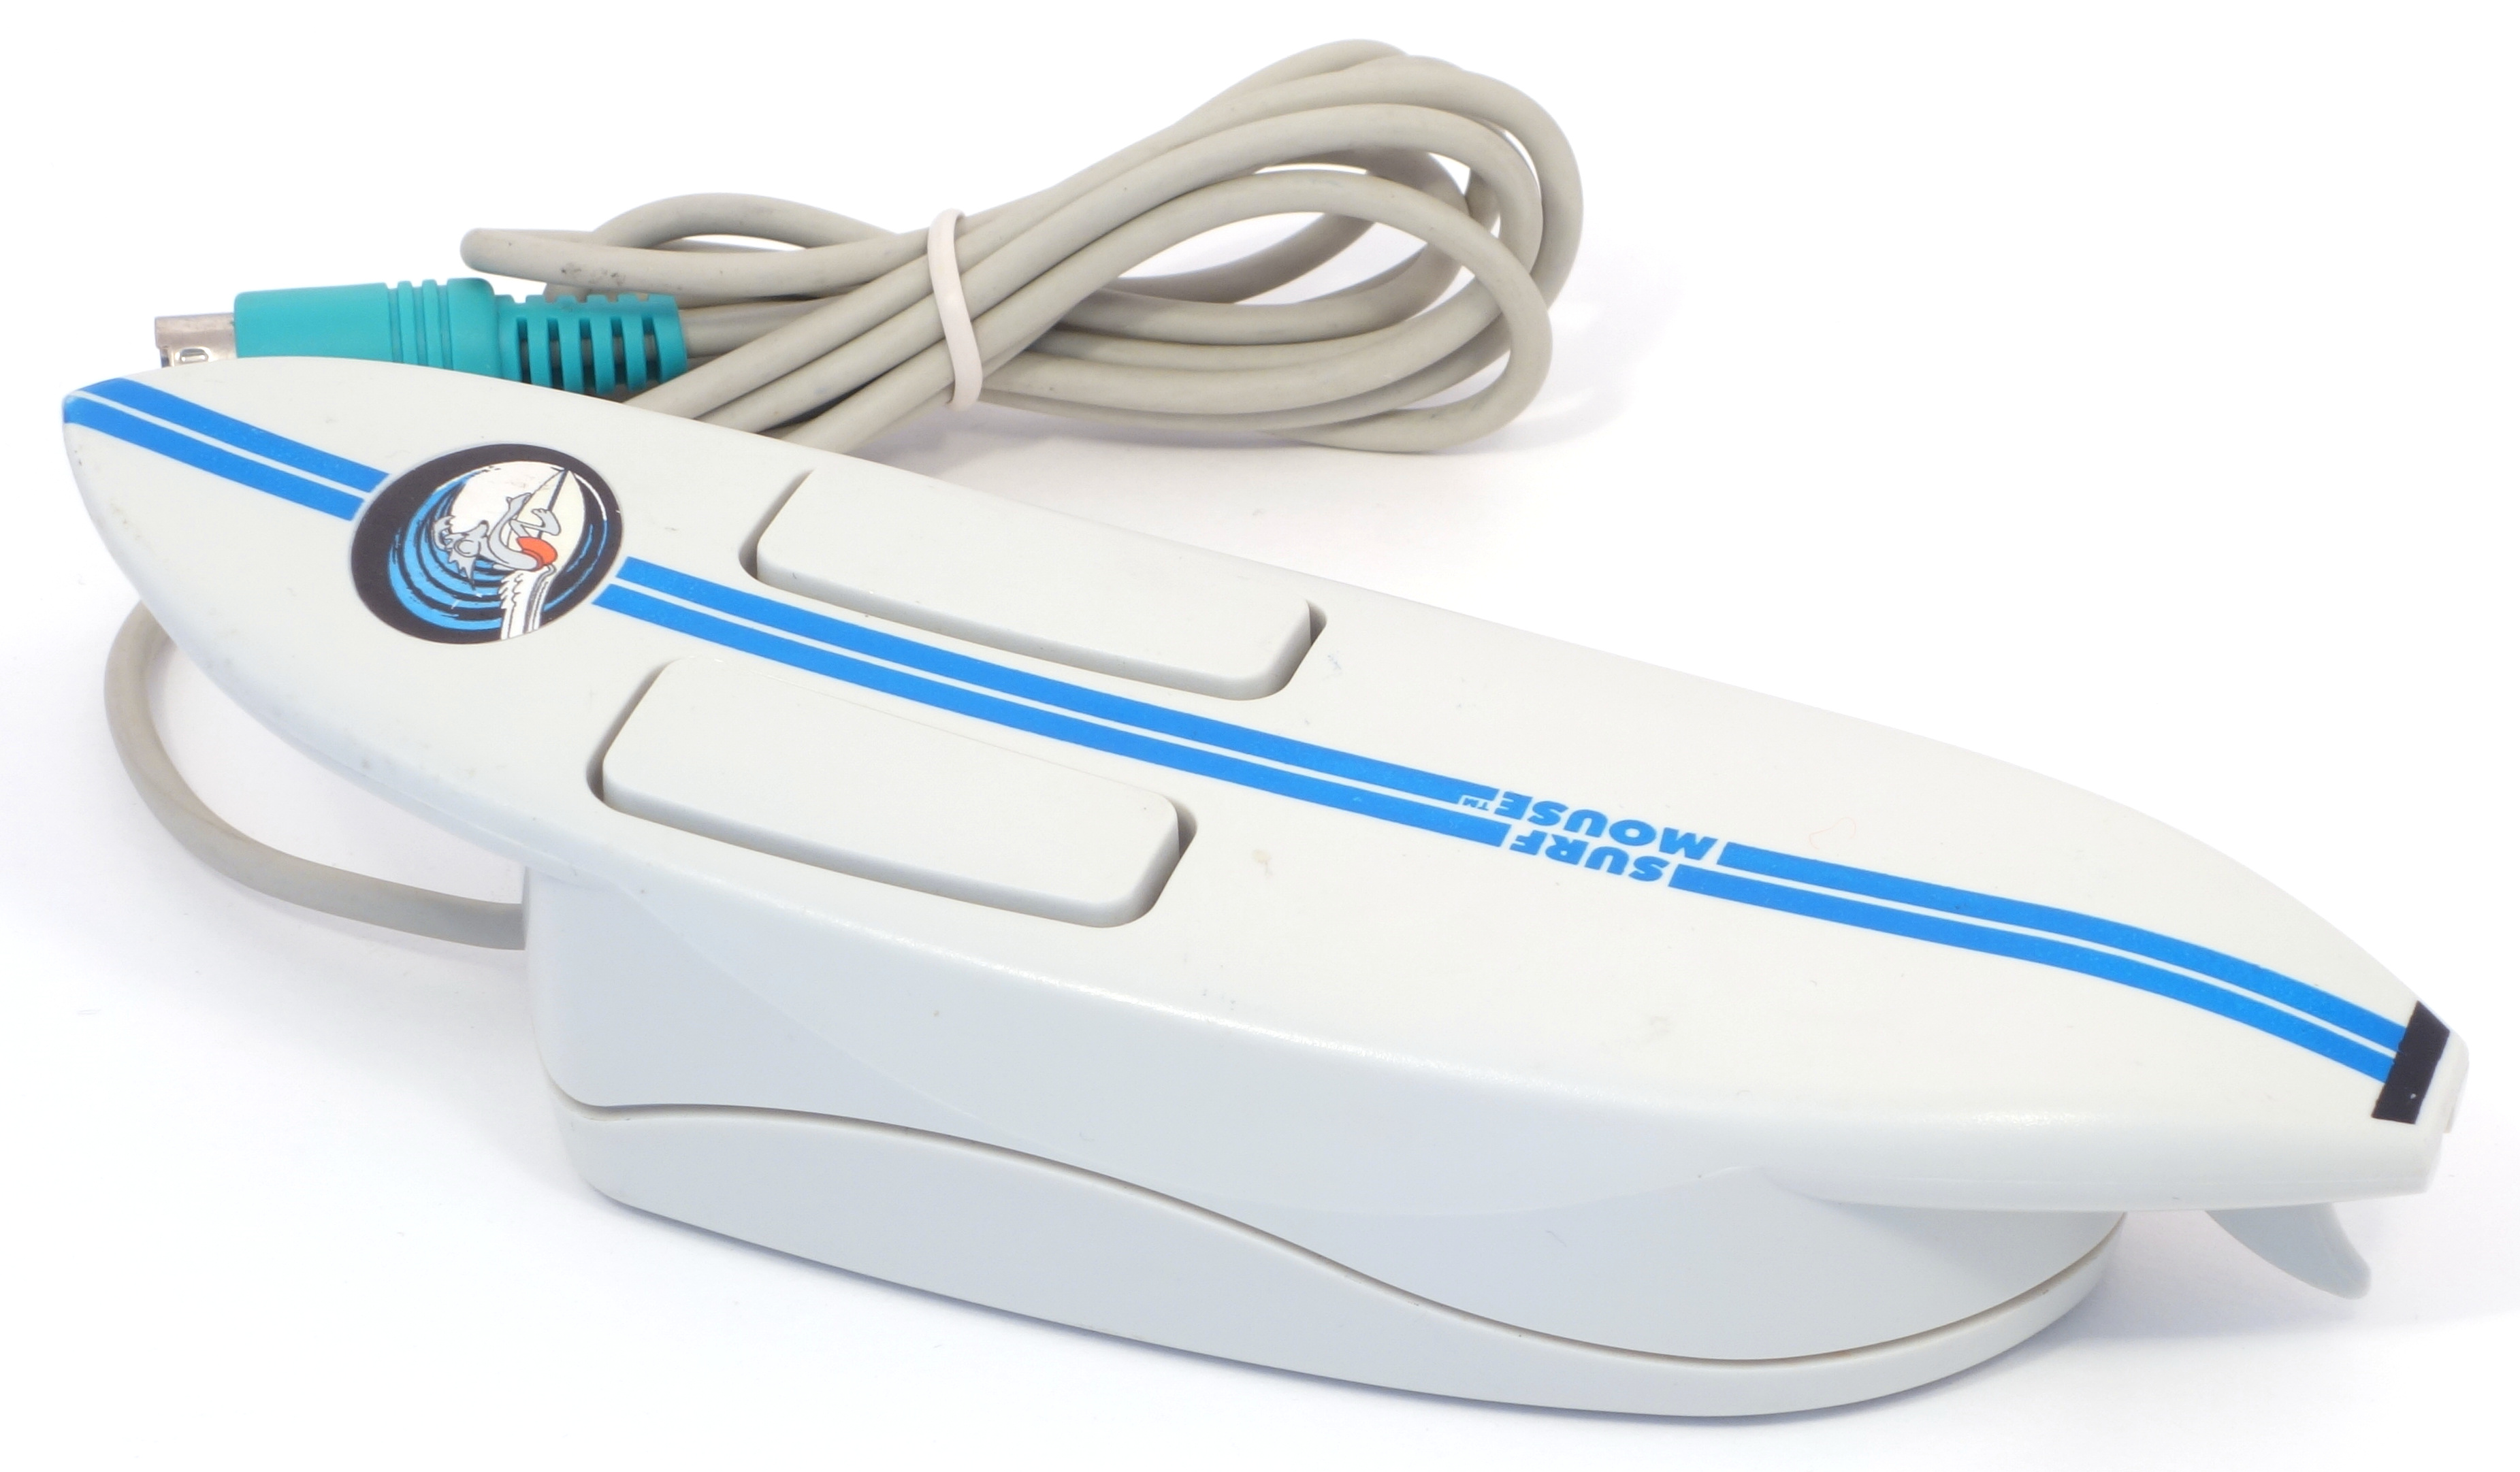
\includegraphics[scale=0.4]{2000_surf_mouse/pic_60.jpg}
    \caption{Мышь SurfMouse}
    \label{fig:SurfMousePic}
\end{figure}

Мышь имеет симметричный корпус, верхней части которого придана форма серфборда. Из-за этого она существенно выдаётся вперед и назад, нависая над основной частью, сохраняющей форму типичной оптомеханической мыши (рис. \ref{fig:SurfMouseTopBottom}). На верхней стороне корпуса присутствуют элементы орнамента с лого SurfMouse, а также две кнопки большого размера. Кнопки расположены ближе к центральной части, чем к передней части корпуса (на самом деле они занимают обычное для мышей положение, а их видимое смещение к центру вызвано исключительно выдающимся вперед носом серфборда).

\begin{figure}[h]
    \centering
    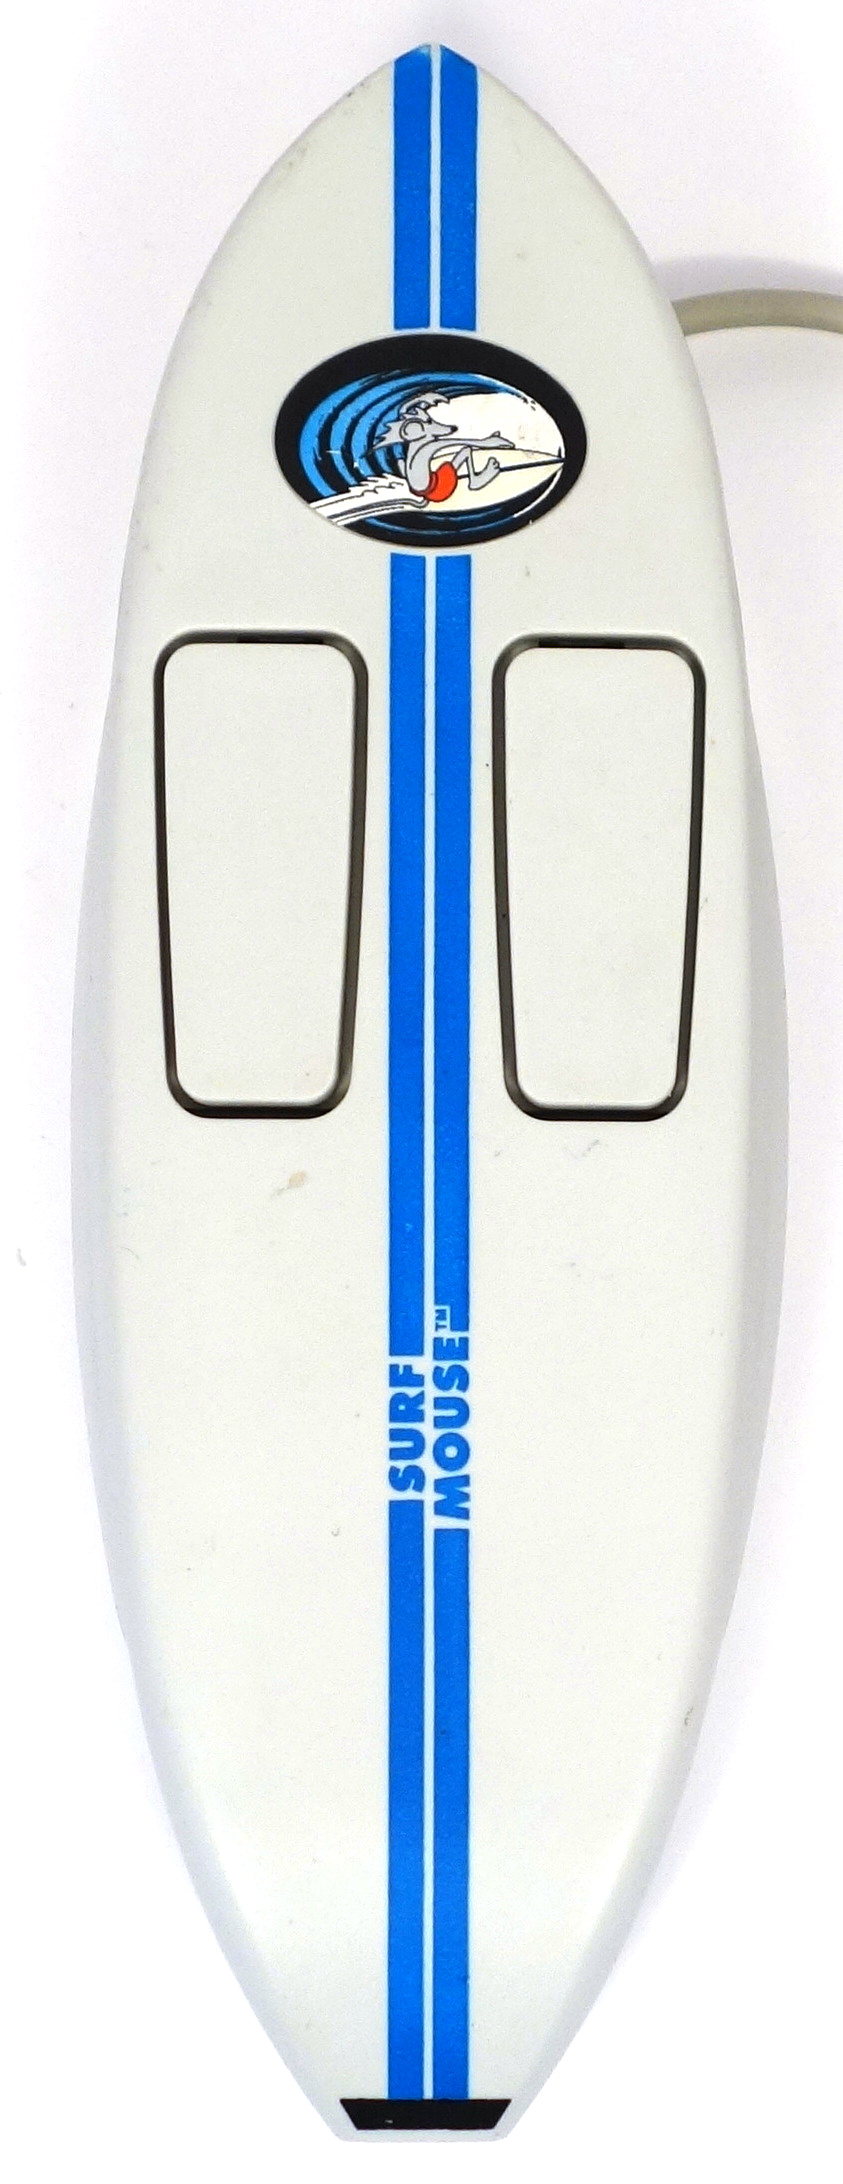
\includegraphics[scale=0.46]{2000_surf_mouse/top_60.jpg}
    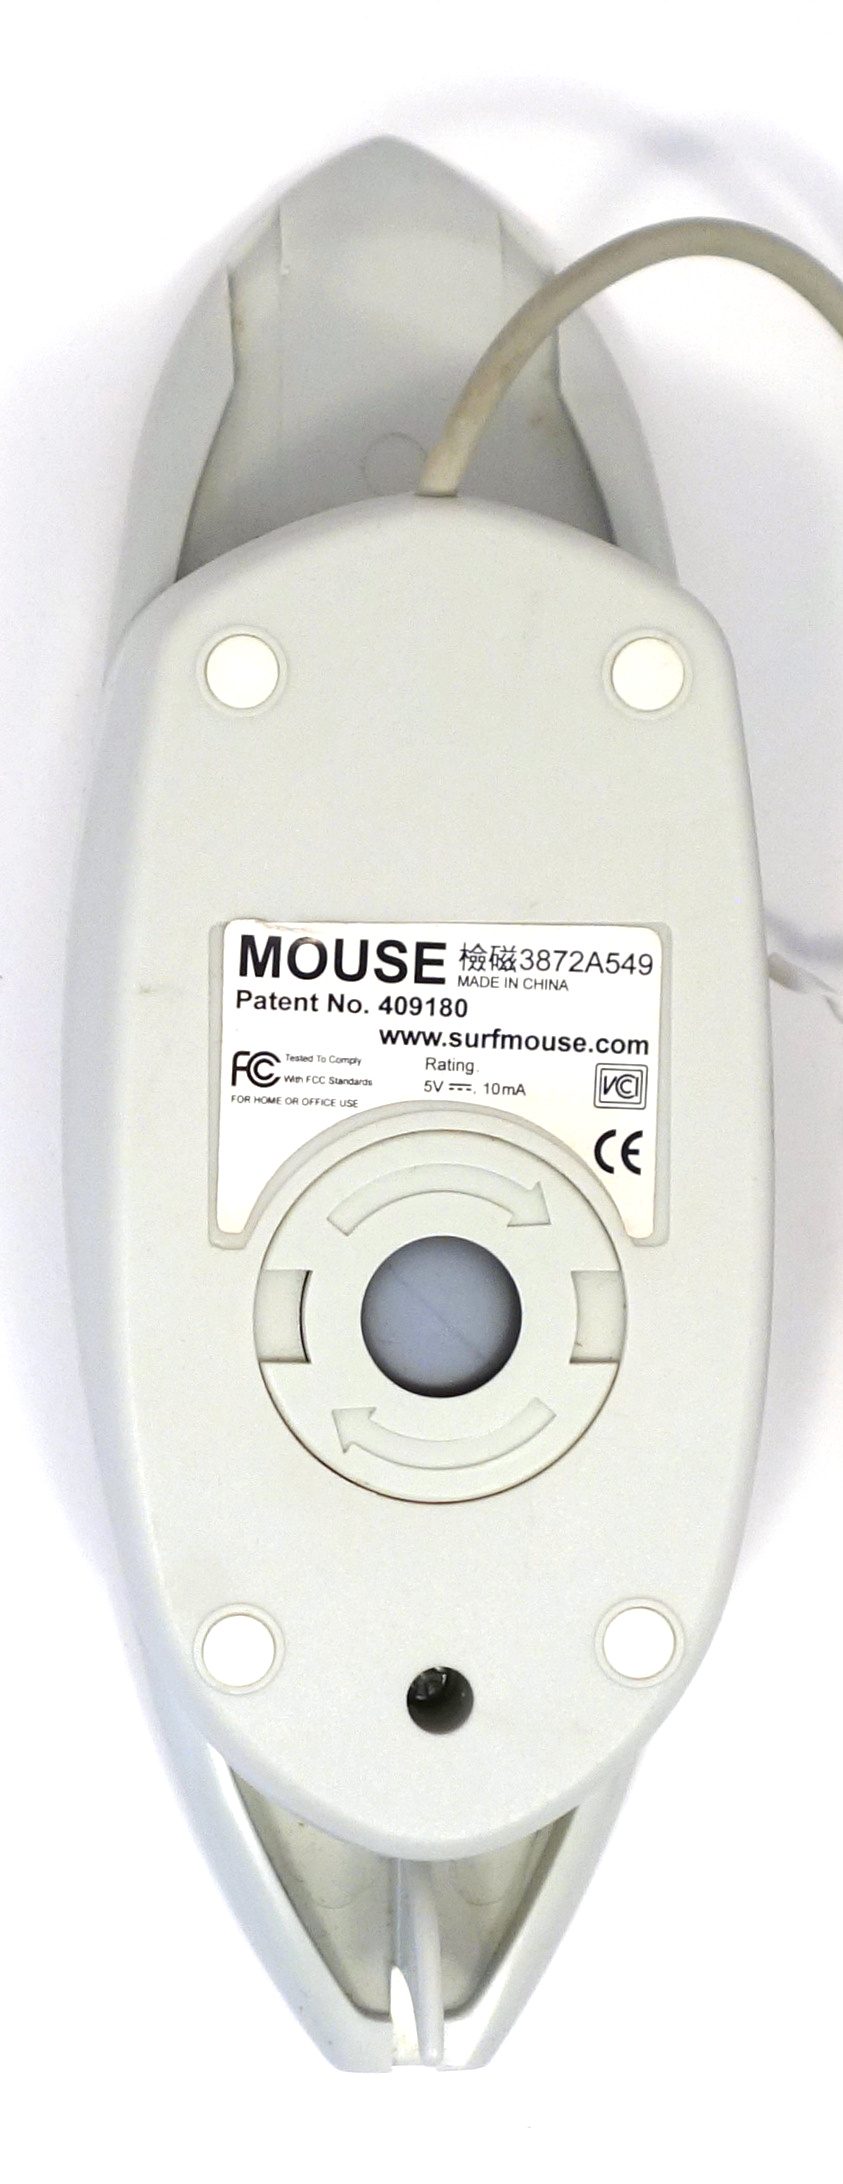
\includegraphics[scale=0.46]{2000_surf_mouse/bottom_60.jpg}
    \caption{SurfMouse, вид сверху и снизу}
    \label{fig:SurfMouseTopBottom}
\end{figure}

Перевернув мышь, можно увидеть традиционные для мышей 90-х годов кольцо-защелку, закрывающее обрезиненный шарик, ножки для скольжения по поверхности, выполненные из низкофрикционного полимера, а также наклейку с маркировкой.

Из-за необходимости копировать форму доски, мышь оказывается крупнее типичных манипуляторов (рис. \ref{fig:SurfMouseSize}) за счет удлиненных передней и задней части.

\begin{figure}[h]
    \centering
    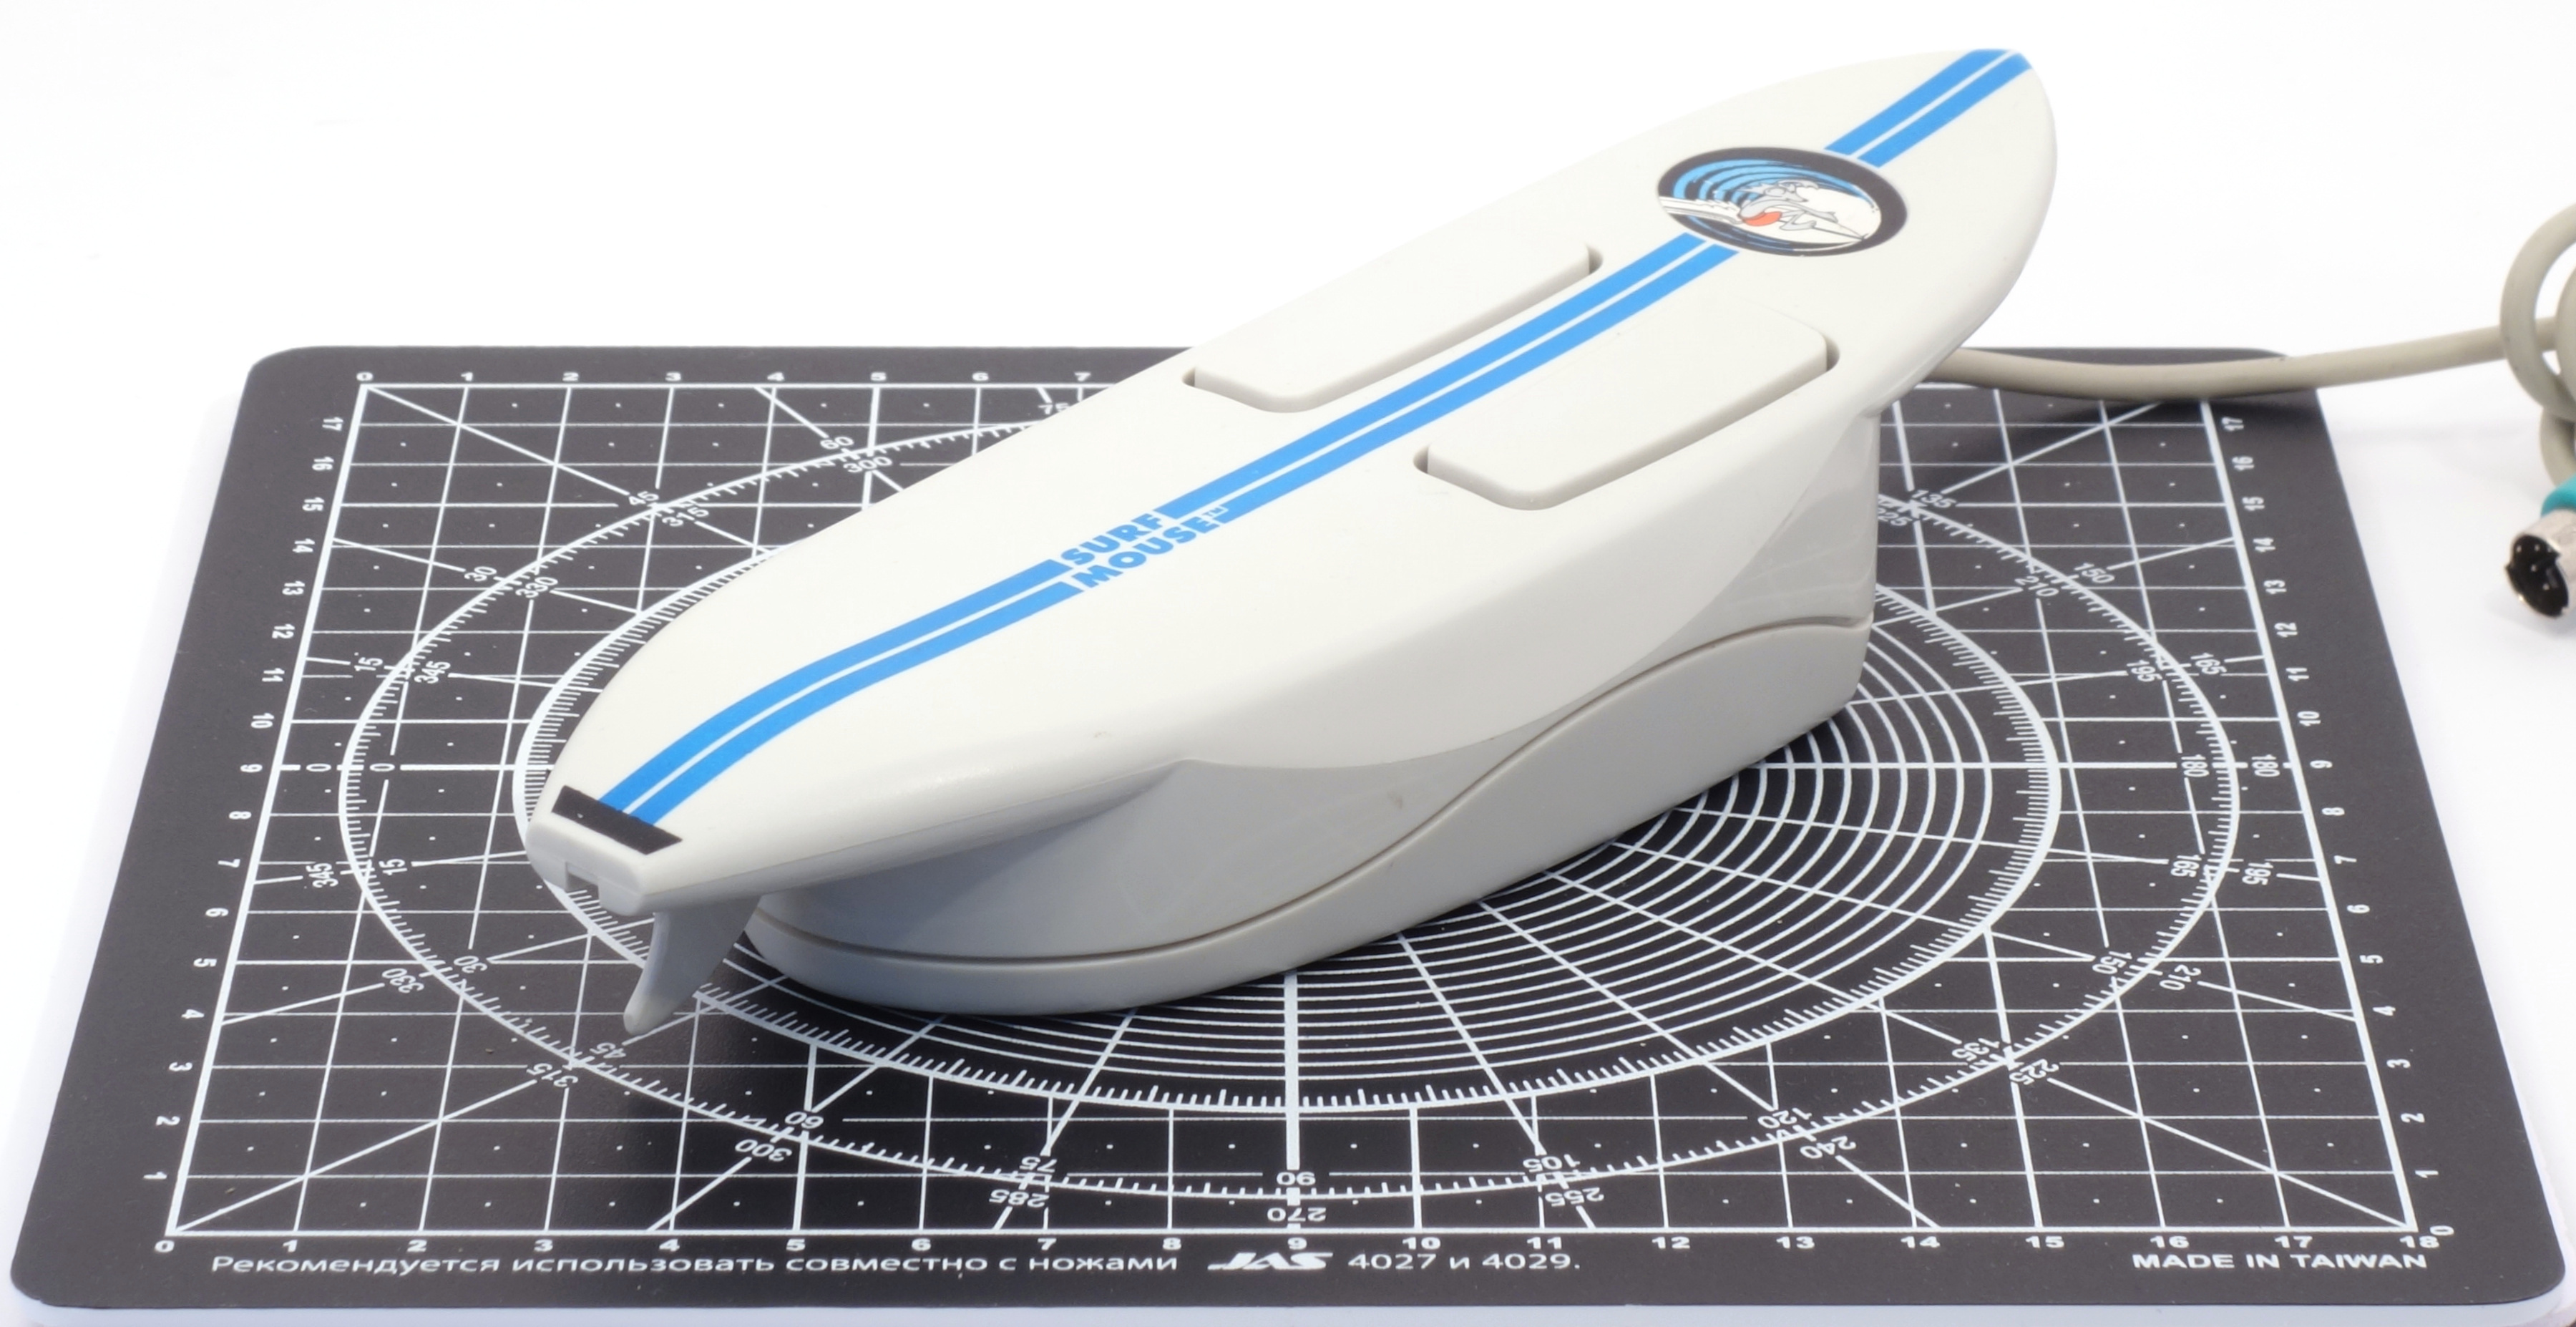
\includegraphics[scale=0.5]{2000_surf_mouse/size_30.jpg}
    \caption{Изображение SurfMouse на размерном коврике с шагом сетки 1~см}
    \label{fig:SurfMouseSize}
\end{figure}

Благодаря симметричности мышь одинаково подходит как для левшей, так и для правшей. Нельзя не заметить, что в целом рука лежит на мыши достаточно удобно (рис. \ref{fig:SurfMouseHand}). Ближняя к пользователю часть <<серфборда>> загнута вниз, образуя удобную горизонтальную подставку под запястье, а расположение кнопок и их форму также можно назвать достаточно удачным.

\begin{figure}[h]
    \centering
    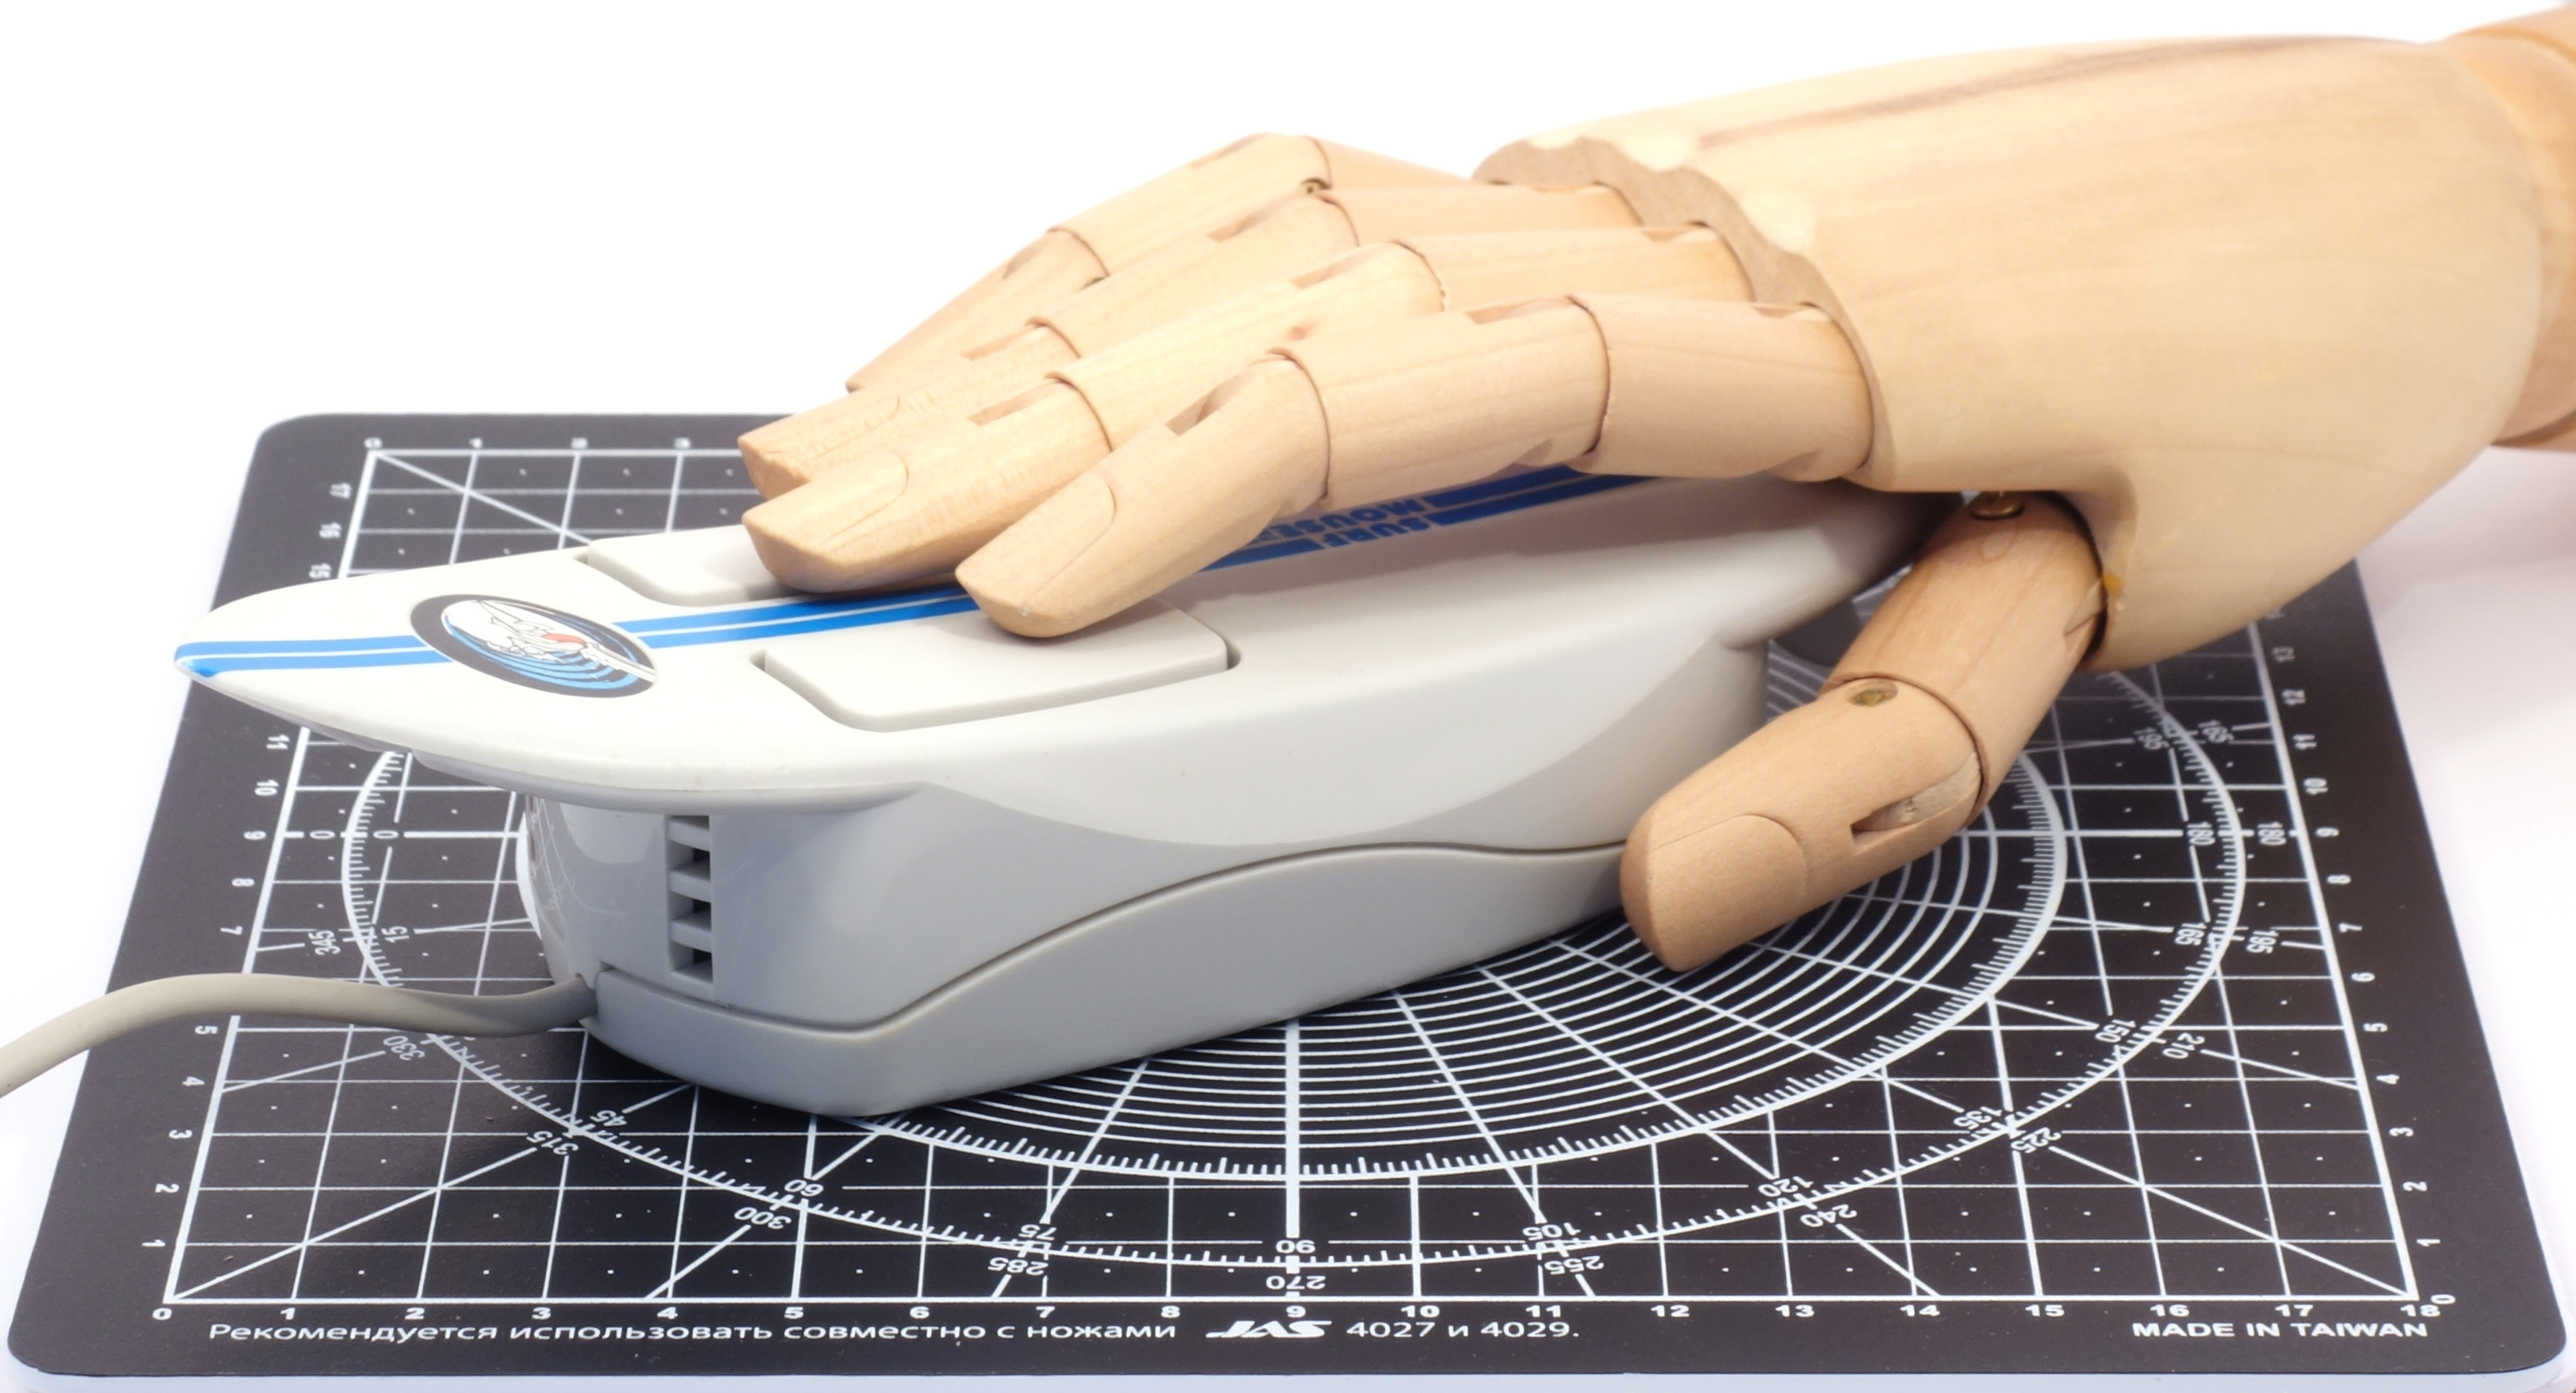
\includegraphics[scale=0.5]{2000_surf_mouse/hand_30.jpg}
    \caption{Изображение SurfMouse с моделью руки человека}
    \label{fig:SurfMouseHand}
\end{figure}

Очевидно, разработчики полагались на хорошую эргономику за счет удобного положения руки на серфборде (специально для этой мыши разработчиками был создан отдельный веб-сайт \url{surfmouse.com} \cite{site}). Однако отсутствие колеса прокрутки, никак не вписывавшегося в стилистику доски для серфинга, в 2000 году уже было критичным недостатком в эргономике мыши.

\begin{figure}[h]
    \centering
    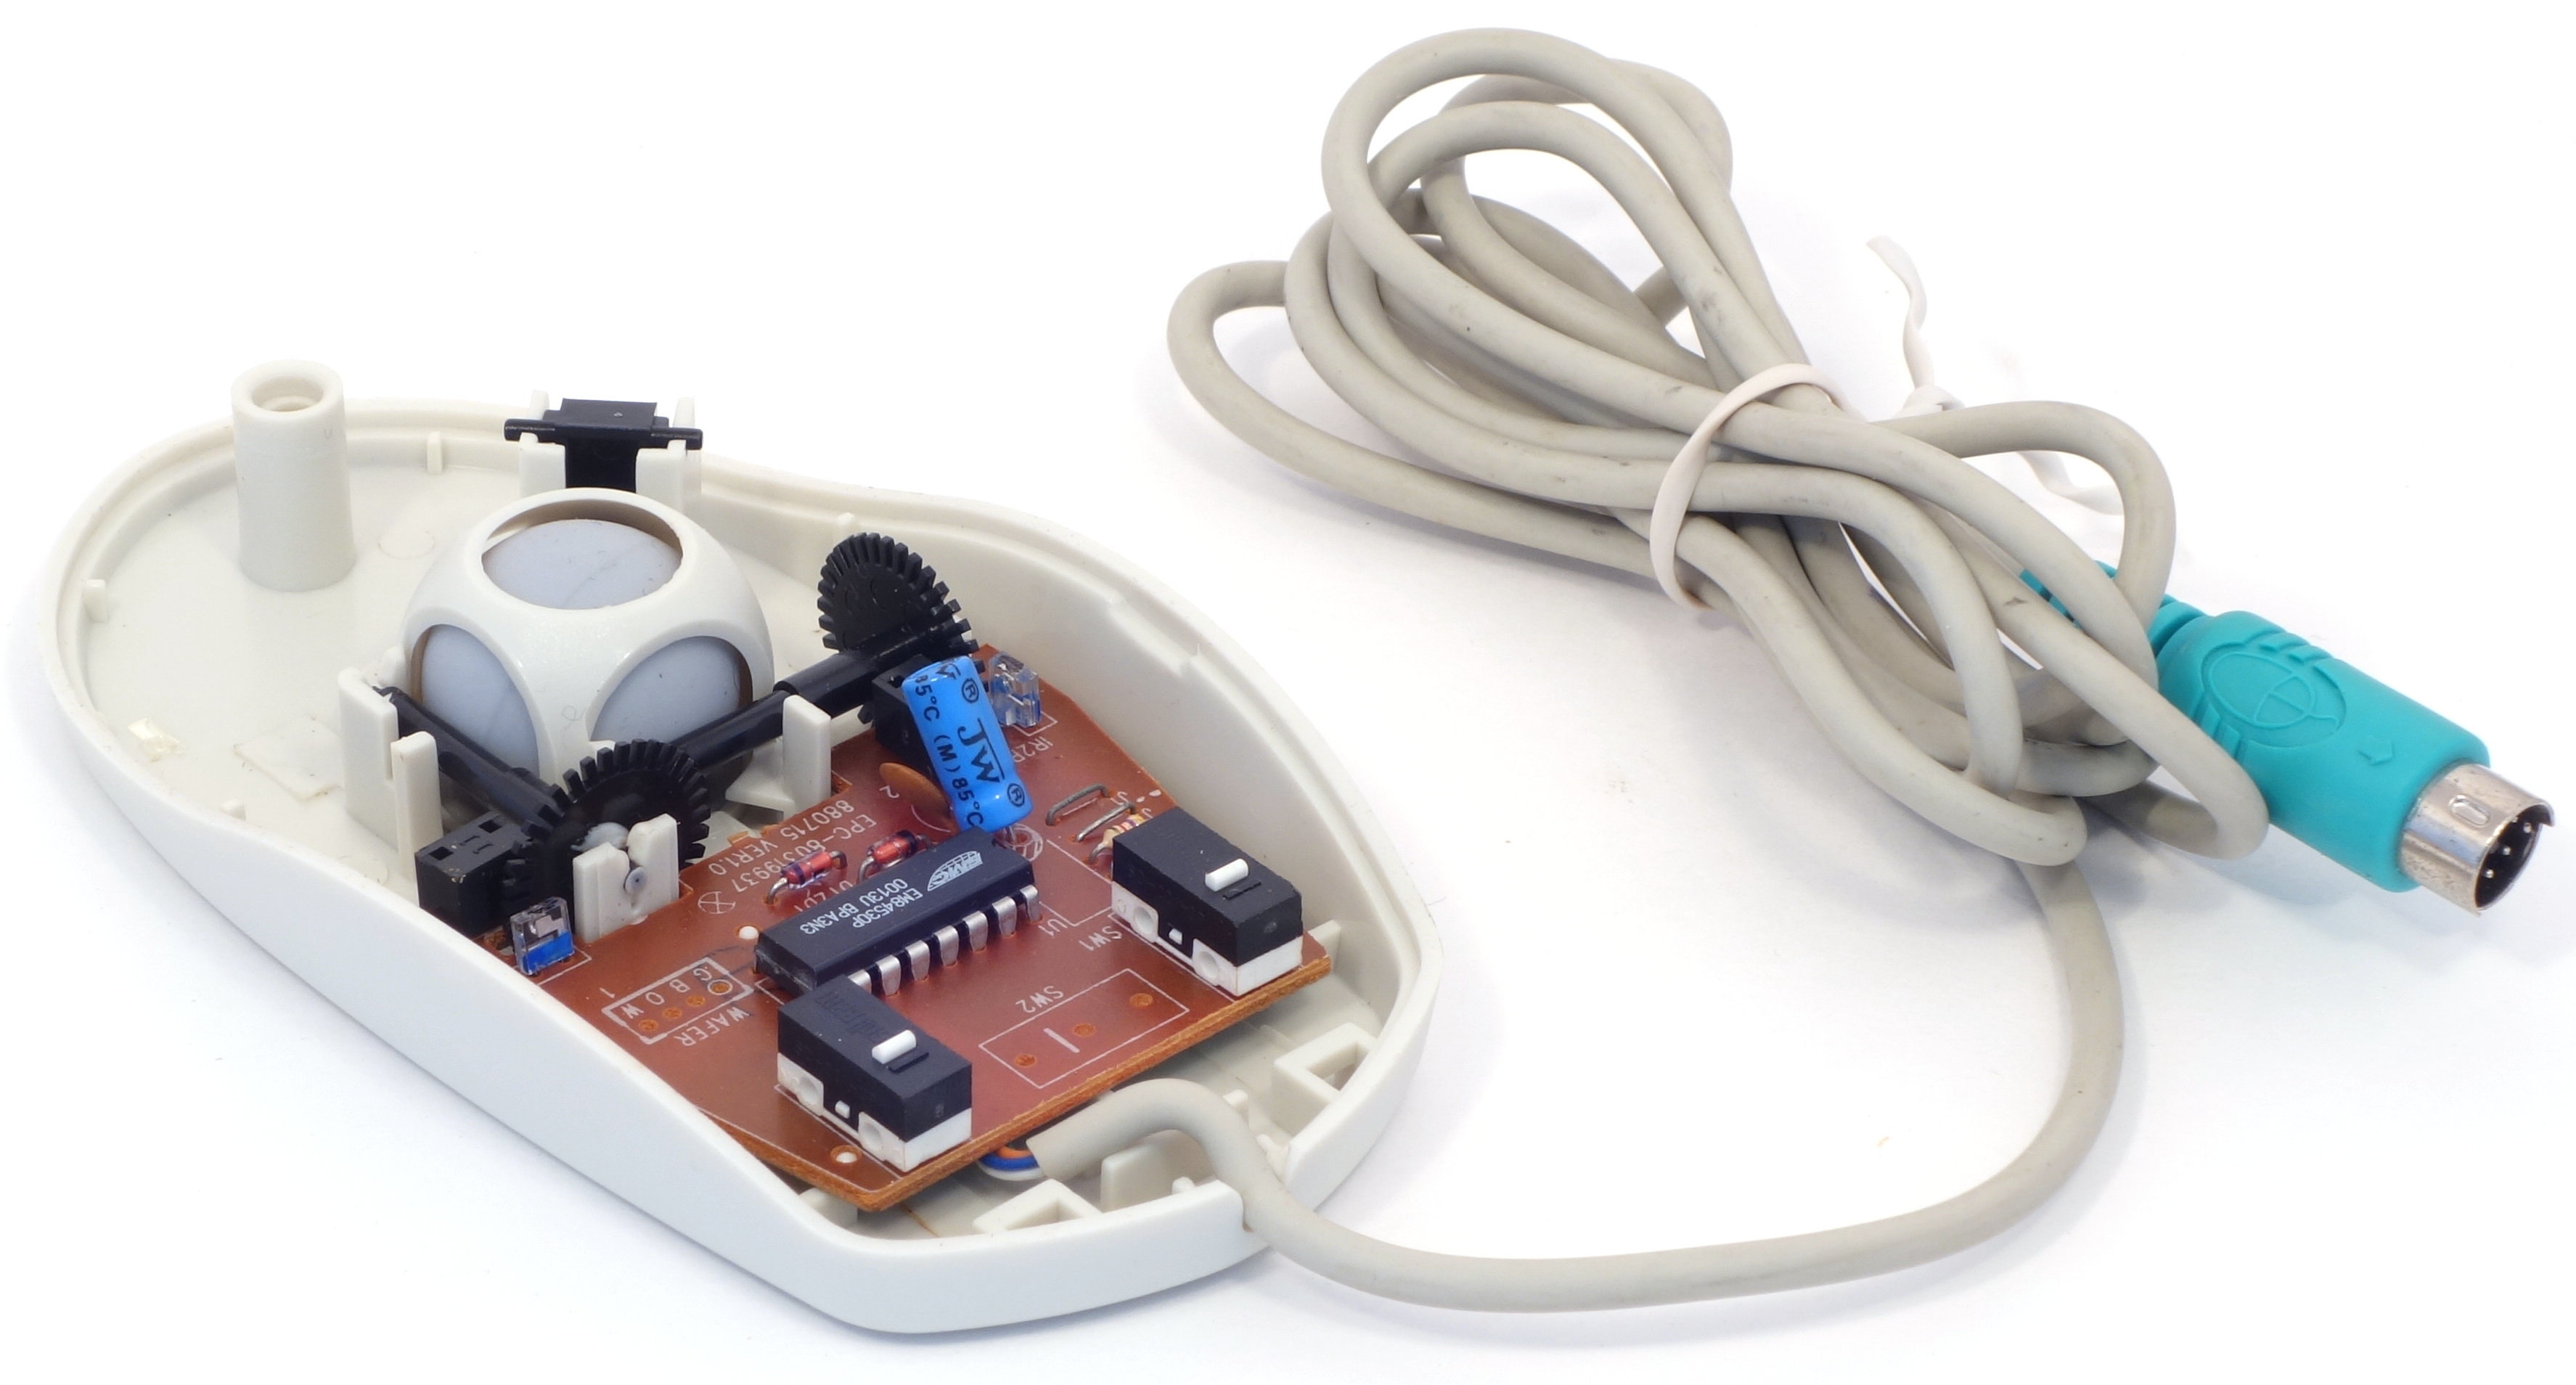
\includegraphics[scale=0.6]{2000_surf_mouse/inside_60.jpg}
    \caption{SurfMouse в разобранном состоянии}
    \label{fig:SurfMouseInside}
\end{figure}

Внутреннее устройство данного манипулятора, показанное на рис. \ref{fig:SurfMouseInside}, открывает типичную оптомеханическую конструкцию первой половины или середины девяностых годов. Более того, представляется вполне вероятным существование в 90-х годах мыши-донора, нижняя часть и наполнение которой послужили основой для SurfMouse.

\begin{thebibliography}{9}
    \bibitem {site} Welcome to SurfMouse.com -- Surf the Web in Style! \url{https://web.archive.org/web/20001204212200/http://www.surfmouse.com/}
\end{thebibliography}

\end{document}
